\documentclass[a4paper,14pt]{extarticle}
\usepackage{../../tex-shared/preamble}

\renewcommand{\mylabnumber}{4}
\renewcommand{\mylabtitle}{Исследование создания mdi-приложений.
Сериализация объектов. Стандартные диалоги}
\renewcommand{\mysubject}{Платформа .NET}
\renewcommand{\mylecturer}{Забаштанский А.К.}

\begin{document}
\begin{titlepage}
    
    \thispagestyle{empty}
    
    \begin{center}
        
        Министерство науки и Высшего образования Российской Федерации \\
        Севастопольский государственный университет \\
        Кафедра ИС
        
        \vfill

        Отчет \\
        по лабораторной работе №\mylabnumber \\
        \enquote{\mylabtitle} \\
        по дисциплине \\
        \enquote{\MakeTextUppercase{\mysubject}}

    \end{center}

    \vspace{1cm}

    \noindent\hspace{7.5cm} Выполнил студент группы ИС/б-17-2-о \\
    \null\hspace{7.5cm} Горбенко К. Н. \\
    \null\hspace{7.5cm} Проверил \\
    \null\hspace{7.5cm} \mylecturer

    \vfill

    \begin{center}
        Севастополь \\
        \the\year{}
    \end{center}

\end{titlepage}

\section{Цель работы}
\begin{itemize}
    \item Изучить особенности разработки MDI-приложений в Visual Studio .Net;
    \item изучить способы сохранения данных в файл и загрузки из файла;
    \item освоить механизм сериализации и десериализации объектов.
\end{itemize}

\section{Задание на работу}
Для варианта № 3 задана следующая схема данных:
\textbf{ПЕЧАТНОЕ ИЗДАНИЕ: название, ФИО автора, стоимость}.
\begin{enumerate}
    \item Создать текстовый редактор NotepadC\#, добавив недостающие пункты меню и функции.
    \item На основании лабораторной работы 3 создать MDI-приложение. Информация в окне
    должна отображаться в виде таблицы. Иметь возможность делать выборку данных по
    различным критериям.
    \item Добавить пункты меню для сохранения объектов в файл и загрузки. При сохранении
    использовать стандартные диалоговые окна и механизм сериализации. В класс добавить
    поле «Дата создания объекта». Поле не сериализовать, а при десериализации заново
    устанавливать по системной дате.
\end{enumerate}

\section{Ход работы}
\subsection{Текстовый редактор Notepad}
Создадим текстовый редактор. Основу текстового редактора составляет элемент
\code{RichTextBox}. \code{RichTextBox} не имеет свойства \code{Text}, поэтому
его нельзя привязать к соответствующему свойству во вью-модели. Решением является
использование сторонней библиотеки, расширяющей \code{RichTextBox}: \code{XceedWpfToolkit}.

Создадим главную страницу приложения:

\begin{lstlisting}
<Page x:Class="Notepad.Views.NotepadControl"
      ...
      xmlns:viewModels="clr-namespace:Notepad.ViewModels"
      xmlns:xceedWpfToolkit="clr-namespace:Xceed.Wpf.Toolkit;assembly=Xceed.Wpf.Toolkit"
      d:DataContext="{d:DesignInstance viewModels:NotepadControlViewModel}">

    <DockPanel LastChildFill="True">
        <Menu DockPanel.Dock="Top">
            <MenuItem Header="File">
                <MenuItem Header="Open" Click="Open" />
                <MenuItem Header="Save" Click="Save"/>
                <MenuItem Header="Save As" Click="SaveAs" />
            </MenuItem>
        </Menu>
        <xceedWpfToolkit:RichTextBox Text="{Binding FileContent, Delay=2000, UpdateSourceTrigger=PropertyChanged}"
                                     ScrollViewer.HorizontalScrollBarVisibility="Auto">
            <FlowDocument PageWidth="3000" />
            <xceedWpfToolkit:RichTextBox.TextFormatter>
                <xceedWpfToolkit:PlainTextFormatter />
            </xceedWpfToolkit:RichTextBox.TextFormatter>
        </xceedWpfToolkit:RichTextBox>
    </DockPanel>
</Page>
\end{lstlisting}

\begin{figure}[H]
    \centering
    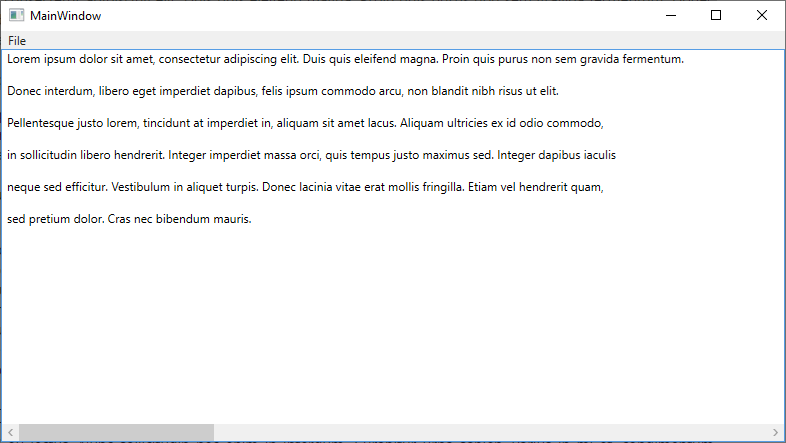
\includegraphics[width=.8\linewidth]{notepad}
    \caption{Текстовый редактор}
    \label{fig:notepad}
\end{figure}

В заголовке страницы импортировано пространство имен включенной в проект библиотеки.
Для компоновки страницы использовался элемент \code{DockPanel} с включенным свойством
\code{LastChildFill}, которое заставляет последний элемент занять все возожное место.
Это использовано для того, чтобы растянуть редактор на все окно.

Ниже приведена логика вызова диалогов выбора файла для открытия и сохранения. Кроме того,
там происходит вызов команд вью-модели.

\begin{lstlisting}
public partial class NotepadControl
{
    public NotepadControl()
    {
        InitializeComponent();
    }

    private void Open(object sender, RoutedEventArgs e)
    {
        var dialog = new OpenFileDialog
        {
            Filter = "All files (*.*) | *.*"
        };

        if (dialog.ShowDialog() != true) return;

        if (DataContext is NotepadControlViewModel viewModel)
        {
            viewModel.OpenCommand.Execute(dialog.FileName);
        }
    }

    private void Save(object sender, RoutedEventArgs e)
    {
        if (DataContext is NotepadControlViewModel viewModel)
        {
            if (string.IsNullOrWhiteSpace(viewModel.FilePath))
            {
                SaveAs(sender, e);
            }
            else
            {
                viewModel.SaveCommand.Execute(null);
            }
        }
    }

    private void SaveAs(object sender, RoutedEventArgs e)
    {
        var dialog = new SaveFileDialog
        {
            Filter = "All files (*.*) | *.*"
        };

        if (dialog.ShowDialog() != true) return;

        if (DataContext is NotepadControlViewModel viewModel)
        {
            viewModel.SaveAsCommand.Execute(dialog.FileName);
        }
    }
}
\end{lstlisting}

Вью-модель представлена на следующем листинге.

\begin{lstlisting}
public class NotepadControlViewModel : INotifyPropertyChanged
{
    private ICommand openCommand;
    private ICommand saveAsCommand;
    private ICommand saveCommand;
    private string fileContent;
    private string filePath;

    public string FileContent
    {
        get => fileContent;
        set
        {
            fileContent = value;
            OnPropertyChanged(nameof(FileContent));
        }
    }

    public string FilePath
    {
        get => filePath;
        set
        {
            filePath = value;
            OnPropertyChanged(nameof(FilePath));
        }
    }

    public ICommand OpenCommand =>
        openCommand ??= new RelayCommand(obj =>
        {
            try
            {
                if (!(obj is string path)) return;

                FileContent = File.ReadAllText(path);
                filePath = path;
            }
            catch
            {
                filePath = string.Empty;
                throw;
            }
        });

    public ICommand SaveCommand => saveCommand ??= new RelayCommand(obj => SaveAsCommand.Execute(filePath));
    public ICommand SaveAsCommand => saveAsCommand ??= new RelayCommand(obj =>
    {
        if (!(obj is string path)) return;

        File.WriteAllText(path, FileContent);
        filePath = path;
    });

    public event PropertyChangedEventHandler PropertyChanged;

    [NotifyPropertyChangedInvocator]
    protected virtual void OnPropertyChanged([CallerMemberName] string propertyName = null)
    {
        PropertyChanged?.Invoke(this, new PropertyChangedEventArgs(propertyName));
    }
}
\end{lstlisting}

В данной вью-модели представлены свойства \code{OpenCommand, SaveAsCommand, SaveCommand,
FileContent, FilePath}. \code{FileContent} и \code{FilePath} представляют содержание
файла и путь к нему соответственно. Содержание обновляется автоматически при изменении
данных в редакторе, путь обновляется только при открытии или сохранении.

Команды \code{OpenCommand, SaveAsCommand, SaveCommand} необходимы для реализации логики
открытия файла и сохранения в файл.

\subsection{Mdi приложение}
Создадим страницу, представляющую форму для изменения списка объектов и их свойств
в виде таблицы. В качестве таблицы используем \code{DataGrid}. Для таблицы создадим
столбцы и свяжем их с соответствующими свойствами печатного издания. Добавим поле даты.
Для удаления печатного издания из таблицы создадим столбец с соответствующей кнопкой.
Разметка страницы представлена далее:

\begin{lstlisting}
<Page Name="PrintedEditionControlPage"
    xmlns:viewModels="clr-namespace:PrintedEditionMdi.ViewModels"
    d:DataContext="{d:DesignInstance viewModels:PrintedEditionControlViewModel}"
    Title="PrintedEditionControl">

    <StackPanel>
        <Menu>
            <MenuItem Header="File">
                <MenuItem Header="Open" Click="OpenButtonClick"></MenuItem>
                <MenuItem Header="Save As" Click="SaveAsButtonClick"></MenuItem>
            </MenuItem>
        </Menu>
        <TextBox Text="{Binding Filter, UpdateSourceTrigger=PropertyChanged}" FlowDirection="RightToLeft" Margin="5"></TextBox>
        <DataGrid HorizontalAlignment="Left"
                    ItemsSource="{Binding PrintedEditions}"
                    SelectedItem="{Binding SelectedItem}"
                    AutoGenerateColumns="False"
                    IsTextSearchEnabled="True">
            <DataGrid.Columns>
                <DataGridTextColumn Binding="{Binding Name}" Width="0.2*" Header="Name" />
                <DataGridTextColumn Binding="{Binding Author}" Width="0.2*" Header="Author" />
                <DataGridTextColumn Binding="{Binding Price}" Width="0.2*" Header="Price" />
                <DataGridTextColumn Binding="{Binding CreatedAt, StringFormat='dd/MM/yyyy'}" IsReadOnly="True"
                                    Width="0.2*" Header="Created at" />
                <DataGridTemplateColumn Width="0.1*">
                    <DataGridTemplateColumn.CellTemplate>
                        <DataTemplate>
                            <Button Command="{Binding Path=DataContext.RemoveCommand,
                                                        ElementName=PrintedEditionControlPage}">Delete</Button>
                        </DataTemplate>
                    </DataGridTemplateColumn.CellTemplate>
                </DataGridTemplateColumn>
            </DataGrid.Columns>
        </DataGrid>
    </StackPanel>
</Page>
\end{lstlisting}

\begin{figure}[H]
    \centering
    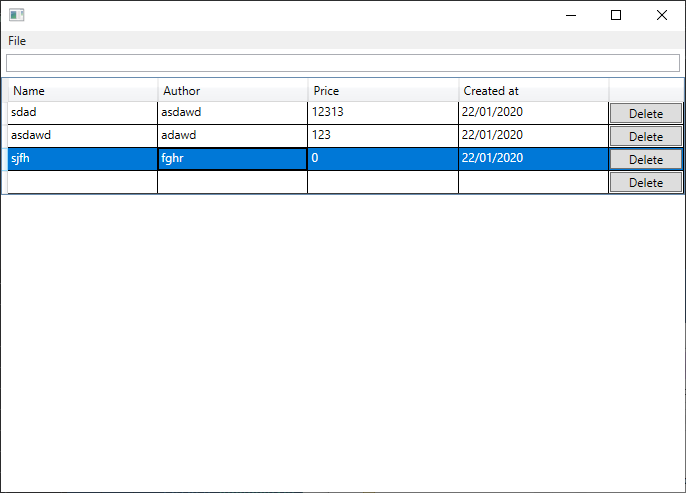
\includegraphics[width=.8\linewidth]{mdi}
    \caption{Приложение редактирования печатных изданий}
    \label{fig:mdi}
\end{figure}

Рассмотрим вызов команд \code{OpenButtonClick} и \code{SaveAsButtonClick}.

\begin{lstlisting}
public partial class PrintedEditionControl
{
    public PrintedEditionControl()
    {
        InitializeComponent();
    }

    private void SaveAsButtonClick(object sender, RoutedEventArgs e)
    {
        var dialog = new SaveFileDialog
        {
            FileName = "PrintedEditions",
            DefaultExt = "json",
            Filter = "Printed edition json (.json)|*.json"
        };

        if (dialog.ShowDialog() != true) return;

        if (DataContext is PrintedEditionControlViewModel viewModel &&
            viewModel.SaveCommand.CanExecute(new object()))
        {
            viewModel.SaveCommand.Execute(dialog.FileName);
        }
    }

    private void OpenButtonClick(object sender, RoutedEventArgs e)
    {
        var dialog = new OpenFileDialog
        {
            Filter = "Printed edition json (.json)|*.json"
        };

        if (dialog.ShowDialog() != true) return;

        if (DataContext is PrintedEditionControlViewModel viewModel &&
            viewModel.OpenCommand.CanExecute(new object()))
        {
            viewModel.OpenCommand.Execute(dialog.FileName);
        }
    }
}
\end{lstlisting}

В данных методах происходит вызов диалогов выбора файла для открытия и для
сохранения в файл. Затем, в случае успешного выбора, вызывается соответствующая
команда вью-модели. Рассмотрим вью-модель.

\begin{lstlisting}
public class PrintedEditionControlViewModel : INotifyPropertyChanged
{
    private readonly ICollectionView printedEditionsView;
    private ObservableCollection<PrintedEdition> printedEditions;
    private PrintedEdition selectedItem;
    private string filter;
    private ICommand removeCommand;
    private ICommand saveCommand;
    private ICommand openCommand;

    public event PropertyChangedEventHandler PropertyChanged;

    [NotifyPropertyChangedInvocator]
    private void OnPropertyChanged([CallerMemberName] string propertyName = null) =>
        PropertyChanged?.Invoke(this, new PropertyChangedEventArgs(propertyName));

    public PrintedEditionControlViewModel()
    {
        printedEditions = new ObservableCollection<PrintedEdition>();
        printedEditionsView = CollectionViewSource.GetDefaultView(printedEditions);
        printedEditionsView.Filter = x =>
        {
            if (string.IsNullOrEmpty(filter)) return true;
            if (!(x is PrintedEdition printedEdition)) return false;

            return printedEdition.ToString().Contains(filter);
        };
    }

    public ObservableCollection<PrintedEdition> PrintedEditions
    {
        get => printedEditions;
        set
        {
            printedEditions = value;
            printedEditionsView.Refresh();
            OnPropertyChanged(nameof(PrintedEditions));
        }
    }

    public PrintedEdition SelectedItem
    {
        get => selectedItem;
        set
        {
            selectedItem = value;
            OnPropertyChanged(nameof(SelectedItem));
        }
    }

    public string Filter
    {
        get => filter;
        set
        {
            if (filter == value) return;

            filter = value;
            printedEditionsView.Refresh();
            OnPropertyChanged(nameof(Filter));
        }
    }

    public ICommand RemoveCommand =>
        removeCommand ??= new RelayCommand(obj => printedEditions.Remove(selectedItem));

    public ICommand SaveCommand =>
        saveCommand ??= new RelayCommand(obj =>
            PrintedEditionSerializeHelper.Serialize(printedEditions, obj as string));

    public ICommand OpenCommand =>
        openCommand ??= new RelayCommand(obj =>
        {
            var currentDateAndTime = DateTime.Now;

            PrintedEditionSerializeHelper.Deserialize(obj as string)
                                            .Select(x => { x.CreatedAt = currentDateAndTime; return x; })
                                            .ForEach(x => PrintedEditions.Add(x));
        });
}
\end{lstlisting}

Для реализации фильтрации используется тип ICollectionView, в котором есть функция
фильтрации. Фильтр задается привязкой к полю в представлении. В командах открытия
и сохранения из файла используется механизм сериализации в Json. Его реализация находится
в классе \code{PrintedEditionSerializeHelper}. Его структура:

\begin{lstlisting}

\end{lstlisting}
public static class PrintedEditionSerializeHelper
{
    public static IEnumerable<PrintedEdition> Deserialize([NotNull] string path)
    {
        if (path == null) throw new ArgumentNullException(nameof(path));

        using var streamReader = File.OpenText(path);
        var json = streamReader.ReadToEnd();

        return JsonConvert.DeserializeObject<PrintedEdition[]>(json);
    }

    public static void Serialize([NotNull] IEnumerable<PrintedEdition> printedEditions, [NotNull] string path)
    {
        if (printedEditions == null) throw new ArgumentNullException(nameof(printedEditions));
        if (path == null) throw new ArgumentNullException(nameof(path));

        var json = JsonConvert.SerializeObject(printedEditions, Formatting.Indented);

        using var streamWriter = new StreamWriter(path);
        streamWriter.Write(json);
    }
}

Данный класс выполняет сериализацию и десериализацию коллекции печатных изданий в Json,
а затем записывает результат в файл.

\section*{Вывод}
В ходе лабораторной работы было создано Mdi-приложение с табличным редактором, возможностью
записи данных в файл и открытием файла. Для создания таблицы использовался элемент
\code{DataGrid}, имеющий возможность привязки данных в таблице к свойству класса C\#.
Для сериализации использовалась библиотека \code{NewtonsoftJson}.

Кроме того, был создан текстовый редактор на основе \code{RichTextBox}.
\end{document}